\chapter{A Declarative Specification Language}\label{dl}
% Not happy with the way Assumption is laid out here, but can't find something I like /more/ than having an rfloor character here.
Noticed in \autoref{teExample} and commented on in \autoref{ci}, we encountered the anomalous constructor \haskell{Assumptions} when building a \haskell{DocDesc}. The \haskell[breakanywhere, breakanywheresymbolpre=\textcolor{black}{-}]{Assumptions} constructor is constant and unlike other \haskell{DocDesc} ``chunk" constructors, such as: \haskell{FReqsSub}, \haskell{LCsProg}, and \haskell{DDs}. The other constructors include an argument concerning the list of chunks to be displayed, whereas \haskell{Assumptions} retrieves the information from the \haskell{ChunkDB} database contained within \haskell{SystemInformation}.

The unique \haskell{Assumptions} \haskell{DocDesc} constructor introduces consistency problems at two separate levels. From a user-facing perspective the constructor is completely inconsistent. There are not any other constructors within \haskell{DocDesc} that omit the chunks to display. There is no user-perceptible \textit{reason} that the \haskell{Assumptions} constructor behaves differently, placing the constructor into a group of ``things that do not make sense but that is the way they are." From a Drasil maintainer perspective, the constructor's unique properties makes it a regular after-thought when designing or implementing components for \textit{drasil-docLang}. We further lose consistency (through unavailability) within generated Drasil documents. The loss of consistency is because for every instance where assumptions are of interest, we are required to re-acquire the chunks from the database, because they are not stored \textit{in} \haskell{DocDesc} and thus not immediately available. An example of the inconsistency caused by the \haskell{Assumptions} constructor is that no generated traceability matrices mention assumptions as they are not available at the time when the dependencies are calculated.

Despite the problems introduced by the \haskell{Assumptions} constructor, it is a desirable addition. The constructor makes a lot of sense when coupled with a \haskell{ChunkDB}. The \haskell{ChunkDB} stores information about the desired system whereas the \haskell{DocDesc} should largely be a high-level declarative language about which sections to include in a requirements document encoding only display-oriented information being pertinent to an SRS. By storing the chunk information in a more accessible place we shift the encoding structure to a more correct approach (an idealized version of Drasil) where the \haskell{SystemInformation} (which contains \haskell{ChunkDB}) knows everything about the system and parts of it are used to generate certain artefacts. By only storing chunks in the database we improve consistency by only having chunks specified in a single location removing opportunities for users to make mistakes, such as having the lists of chunks differ from one another when specified in multiple places.

With the \haskell{Assumptions} constructor being desirable, we examine \haskell{DocDesc} for other constructors that should not explicitly specify their chunks before constructing possible designs. From \autoref{teExample}, we have \haskell{DDs}, \haskell{FReqsSub}, and \haskell{LCsProg} as constructors that take an explicit list of chunks as an argument. In the same structure as \haskell{DDs} there is \haskell{GDs}, \haskell{IMs}, and \haskell{TMs}, which also take a list of chunks. In a similar data structure --- with a similar name --- to \haskell{FReqsSub} is \haskell{NonFReqsSub}. Semantically similar to \haskell{LCsProg} is \haskell{UCsProg}, which provides the unlikely changes section. There are a total of eight constructors that take a list of chunks as an argument where the chunks also exist in the \haskell{ChunkDB}. We aim to standardize how this style of \haskell{DocDesc} constructor behaves and is exposed to a user.

At present, the interactions used to achieve consistency between the \linebreak\haskell{DocDesc} constructors mentioned and \haskell{ChunkDB} is unclear and assigned to the user to ensure. The existing method for non-\haskell{Assumptions} constructors is to either specify the chunks in the constructor as well as specify them explicitly in the correct \haskell{ChunkDB} field, or use functions similar to \haskell{getTraceMapFromDD} (depending on the chunk type) to gather the chunks from the \haskell{DocDesc} constructors and place the returned list in the \haskell{ChunkDB}. Neither of these existing methods make much sense. They further force responsibilities onto users rather than doing what Drasil is designed to do: automate away common errors and inconsistencies!

\section{Making \haskell{Assumptions} Consistent}\label{diFraming}
We have already hinted at a desired solution; one where \haskell{ChunkDB} stores the knowledge and \haskell{DocDesc} describes what and how to display information in an SRS artefact. If we model the desired user experience for the eight constructors after what exists with \haskell{Assumptions} we will remove the argument containing the list of chunks to display and pull that information from a \haskell{ChunkDB} when needed. This is an excellent start! However, we have noted a shortcoming with the \haskell{Assumptions} constructor; namely the chunks are not alway present when needed. One solution is to introduce smart constructors for the data constructors of interest that instantiate the data constructors with an empty list of chunks that is later populated when \haskell{DocDesc} processing occurs. The delayed population of chunks in data constructors invites opportunities for situations where it is unclear if a passed \haskell{DocDesc} has chunks populated or not, forcing an odd mental model for contributors of \textit{drasil-docLang}.

Instead of the delayed population approach, we create the notion of a user-facing declarative language that is traversed and ``expanded" into \haskell{DocDesc}. The user-facing structure contains all information required to generate an SRS. With a multi-step approach to document generation we can allow the user-facing document to diverge from the internal representation and create additional intermediary structures in the future to further enhance and automate document generation as needed. The new structure, named \haskell{SRSDecl} (\textbf{SRS} \textbf{Decl}aration), allows for the constructor design we desire and improves on a deficiency prevalent with the existing \haskell{Assumptions} constructor.

Beginning the process of realizing \haskell{SRSDecl}, we make \haskell{DocDesc} consistent for the planned changes and add a \haskell{[ConceptInstance]} argument to the \haskell{Assumptions} constructor. If we are improving the user interface for constructing SRS documents, we should address the odd \haskell{TraceabilityProg} constructor used to create the traceability matrix section as well because \haskell{SRSDecl} sheds the baggage of \haskell{DocDesc}'s encoding of information.

\section{Tracing Troubles}\label{dlTraceMat}
Although it seems like a tangent, the traceability matrix \haskell{DocDesc} constructor is too concrete and final, while the method to generate a traceability matrix itself is inflexible and requires extraneous work from a user.

To briefly review, the traceability matrix constructor is specified in \autoref{teExample} with:

\begin{tcolorbox}
\begin{minted}{haskell}
TraceabilitySec $ TraceabilityProg [traceTable] [foldlSent
    S "items with each other"]] [LlC traceTable] []
\end{minted}
\end{tcolorbox}

The signatures for \haskell{TraceabilitySec} and \haskell{TraceabilityProg} are:

\begin{tcolorbox}
\begin{minted}{haskell}
type DocDesc = [DocSection]

data DocSection =
  ...
  | TraceabilitySec TraceabilitySec
  ...

data TraceabilitySec = TraceabilityProg [LabelledContent]
  [Sentence] [Contents] [Section]
\end{minted}
\end{tcolorbox}

For the arguments to \haskell{TraceabilityProg}, the \haskell{[LabelledContent]} argument is the same value as the \haskell{[Contents]} of the third argument. The \haskell{LabelledContent} argument is used to created references to individual matrices in the introduction of the traceability section to provide context. The second argument, \haskell{[Sentence]}, is a description of each matrix, the third argument is each matrix (copied verbatim into the generated document), and the final argument is for ``other" content to be copied verbatim --- originally for manual traceability graphs, however, no bundled example provides a traceability graph. The argument arrangement makes little sense, and the duplicated (albeit slightly modified) specification of the traceability matrices themselves is awkward and easily derivable from one or the other.

We discourage manual creation and maintenance of traceability information due to the difficulties to accurately reflect the state of the document, the tediousness of the task, and the time consumed attempting. These reasons are why Drasil implements the function \haskell{generateTraceTable}. Its purpose is to generate a traceability matrix from an SRS, eliminating the need for a human to concern themselves with it. The idea that we can create a traceability matrix automatically largely invalidates the need to manually specify arguments one and three. One issue surrounding \haskell{generateTraceTable}: the function creates a single traceability matrix without any configuration, best described as ``everything against everything." This sort of configuration can be overwhelming and not overly apparent about what useful information it provides. It would be nice to create smaller matrices where we can track dependence of chunks on various assumptions, how knowledge is refined and instantiated, among other configurations to emphasize certain relationships for a given software solution expressed in Drasil. Even better would be to expose the ability for users to select the matrix configurations to include in an SRS. This may seem counterintuitive and unrelated to what we discussed previously about \haskell{generateTraceTable} invalidating two arguments in \haskell{TraceabilityProg}; however, the constructor should be higher-level where the user specifies their ``views" of dependencies that \textit{drasil-docLang} will use to generate traceability matrices (i.e. \haskell{generateTraceTable} should be performed by \textit{drasil-docLang} as needed). 

The final issue with the existing traceability matrix --- shown in \autoref{fig:traceBefore} --- is small from a solution standpoint but something that impedes interpretation of the matrix in the generated documents: the traceability matrix currently does not order the items in any particular way. The lack of sensible ordering makes it difficult to locate a particular item at a glance and makes quickly checking if an item has a given dependency a non-instantaneous task.

\begin{figure}[H]
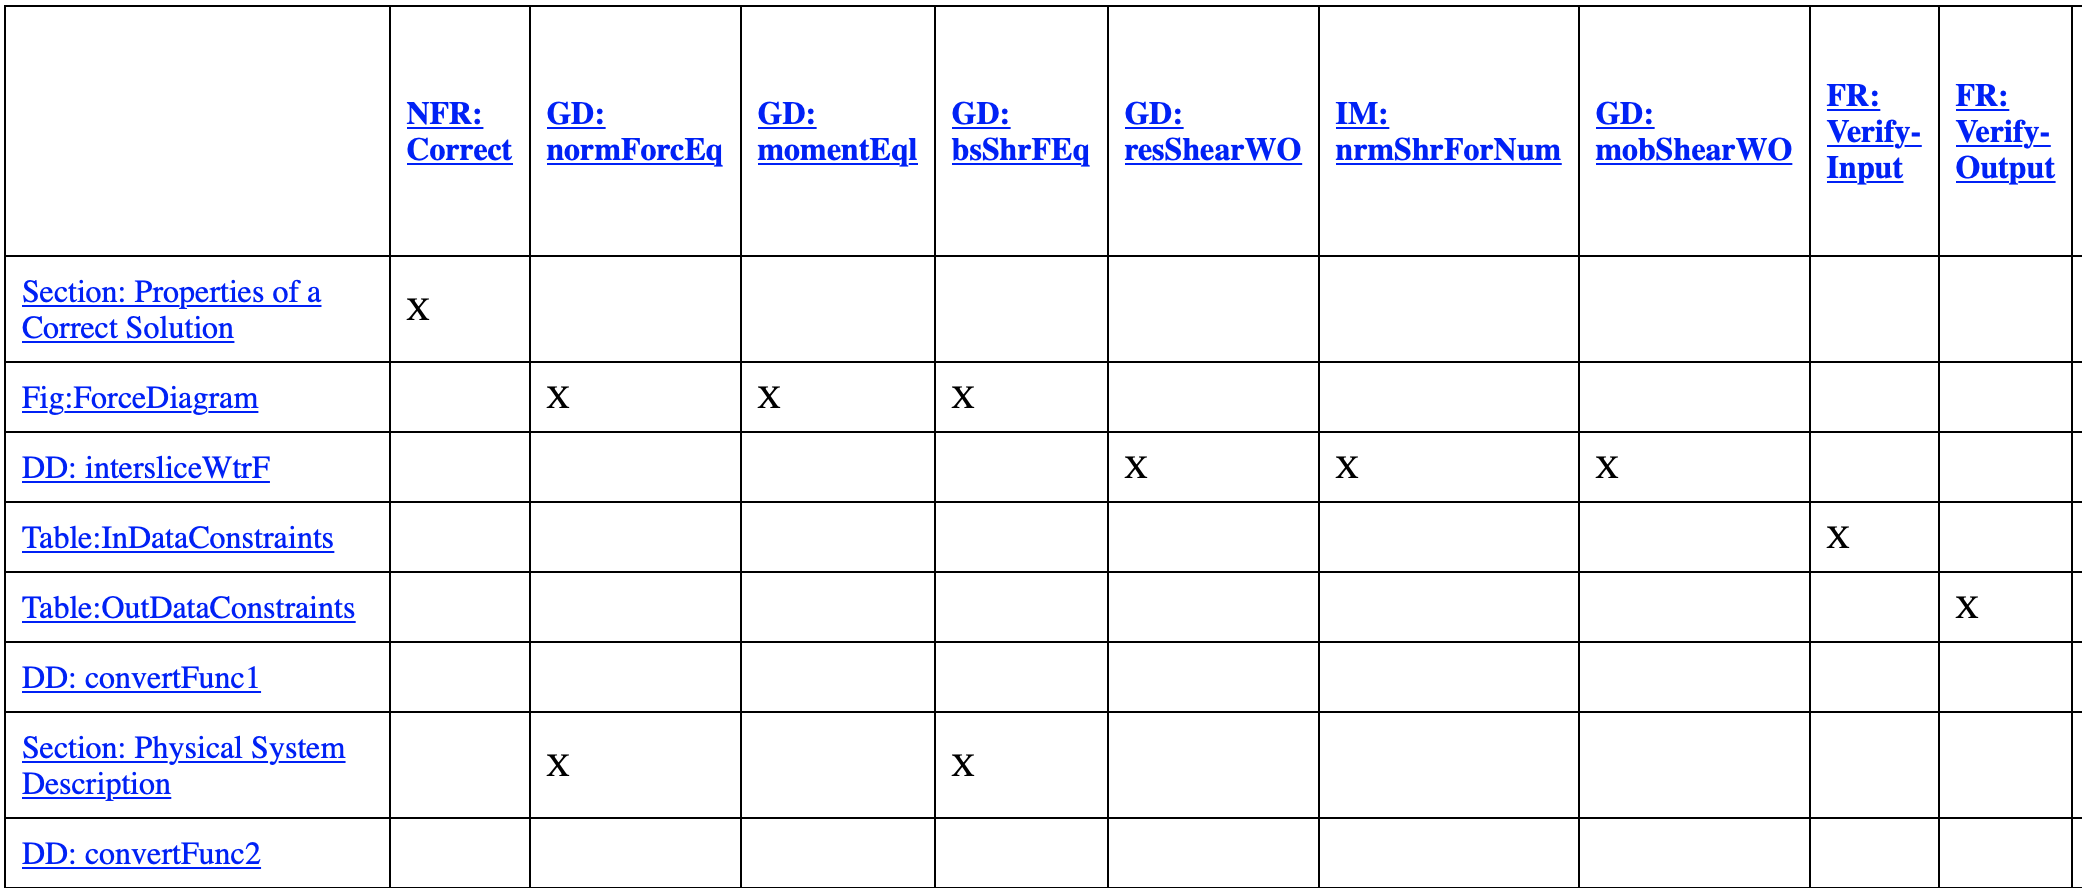
\includegraphics[width=\textwidth]{TraceBefore}
\caption{A portion of the automated traceability matrix for the Drasil example Slope Stability analysis Program (SSP).}\label{fig:traceBefore}
\end{figure}


%% Traceability matrix view design here
We mentioned a solution that introduces ``views" to a traceability matrix. Ideally we would like a constructor where we specify a list of chunk categories (i.e. assumptions, data definitions, etc.) where the list itself can be thought of as a one-dimensional view of a traceability matrix. The user facing syntax for such a constructor could be:

\begin{tcolorbox}
\begin{minted}{haskell}
TraceProg [{-Columns-} viewAssump]
  [{-Rows-} viewReqs, viewLikelyChgs]
\end{minted}
\end{tcolorbox}

When \haskell{TraceProg} is evaluated, \haskell{viewAssump}, \haskell{viewReqs}, and \haskell[breakanywhere, breakanywheresymbolpre=\textcolor{black}{-}]{viewLikelyChgs} are evaluated to retrieve traceability information that is then combined into a complete matrix. The constructor \haskell{TraceProg} addresses the issues described with the existing \haskell{TraceabilityProg} and \haskell{generateTraceTable} implementation thus eliminating the need for a user to perform specific incantations to create a traceability matrix. \haskell{TraceProg} enforces the content present in a traceability section is traceability related. Further, such a constructor inherently adds a sense of ordering and grouping to the displayed items within a matrix. Finally, such a generic \haskell{TraceProg} description allows for specification of many differing (even within the same document) matrices.

With a general guiding design of what we desire as a user-facing interface, we turn our attention to how \haskell{generateTraceTable} builds the traceability matrix. Most of the cross-referencing and chunk dependency tracking is performed by the following two functions: \haskell{generateTraceMap} and \haskell{generateRefbyMap}. These two functions produce tables that are added to \haskell{ChunkDB} and accessible through the \haskell{traceTable} and \haskell{refbyTable} fields, respectively. The information collected in these tables is accurate; we are adjusting the processes with which the information is displayed and organized from these tables in a more human-friendly manner.

%At the core of the single generated matrix is \haskell{traceMRow} and \haskell{traceMCol} which extract chunk \haskell{UID}s in a given dimension:

% \begin{tcolorbox}
% \begin{minted}{haskell}
% traceMRow :: ChunkDB -> [UID]
% traceMRow = nub . Map.keys . (^. refbyTable)
% 
% traceMCol :: ChunkDB -> [UID]
% traceMCol = nub . concat . Map.elems . (^. refbyTable)
% \end{minted}
% \end{tcolorbox}

%The keys of \haskell{refbyTable} are the \haskell{UID}s of chunks which are referred to, referees if you will. The values of \haskell{refbyTable} are the referrers to a given referee. With the current names (and subsequent uses) of \haskell{traceMRow} and \haskell{traceMCol}, we are transposing the idea of how we usually reason about tables: indepedent information along the top (and thus columns). Further the names of the functions do not provide enough meaningful context as someone or some cultures may prefer referrers to be along the top, we will rename \haskell{traceMRow} to \haskell{traceMReferees} and \haskell{traceMCol} to \haskell{traceMReferrers} to be more explicit and layout agnostic.

%With a list of \haskell{UID}s we have four methods to extract a reference from the lists and dependency information:

%\begin{tcolorbox}
%\begin{minted}{haskell}
%traceMHeader :: (ChunkDB -> [UID]) ->
%  SystemInformation -> [Sentence]
%traceMHeader f c = map (`helpToRefField` c) $ f $ _sysinfodb c
% 
%traceMRowHeader :: SystemInformation -> [Sentence]
%traceMRowHeader = traceMHeader traceMReferrers
%
%traceMColHeader :: SystemInformation -> [Sentence]
%traceMColHeader = traceMHeader traceMReferees
%
%traceMColumns :: ChunkDB -> [[UID]]
%traceMColumns c = map (`refbyLookup` (c ^. refbyTable)) $
%  traceMReferees c
%\end{minted}
%\end{tcolorbox}
%
%where \haskell{helpToRefField} is a function taking a \haskell{UID} and returns a \haskell{Ref} \haskell{Sentence} constructor. Finally, we examine how \haskell{generateTraceTable} uses these functions to create a traceability matrix:

%\begin{tcolorbox}
%\begin{minted}{haskell}
%generateTraceTable :: SystemInformation -> LabelledContent
%generateTraceTable c = llcc (makeTabRef "Tracey") $ Table
%  (EmptyS : (traceMColHeader c)) (makeTMatrix
%  	(traceMRowHeader c) (traceMColumns $ _sysinfodb c) $
%  	traceMReferrers $ _sysinfodb c)
%  (showingCxnBw traceyMatrix $ titleize' item +:+
%  	S "of Different" +:+ titleize' section_) True
%\end{minted}
%\end{tcolorbox}

%where \haskell{makeTMatrix} takes a list of row names, a list of all \haskell{UID}s referred to by each row, and a list of all \haskell{UID}s appearing in a column. The output of \haskell{makeTMatrix} is a row major two-dimensional list containing an ``X" in all cells where the row depends on a column. The \haskell{Table} constructor (a part of \textit{drasil-lang}'s \haskell{Content} data structure) takes a list of column headers followed by the row-major matrix contents, a label describing the table, and a boolean indicating whether to display the name of the table. Finally, the \haskell{makeTabRef} and \haskell{llcc} functions make the table referable --- using the \haskell{UID} ``Tracey" --- such that it conforms to the \haskell{TraceabiliyProg} constructor.

%We have mentioned our traceability matrix is transposed, based on the description of the arguments for \haskell{makeTMatrix}, the final argument is a list of columns, however in our case \haskell{traceMReferees} is the list of columns, whereas we're passing \haskell{traceMReferrers}. Further, the second argument ought to be row-major, however \haskell{traceMColumns} is column-major. Remedying these two issues results in:

%\begin{tcolorbox}
%\begin{minted}{haskell}
%traceMColumns :: ChunkDB -> [[UID]]
%traceMColumns c = map (flip traceLookup (c ^. traceTable)) $
%  traceMReferrers c
%
%generateTraceTable :: SystemInformation -> LabelledContent
%generateTraceTable c = llcc (makeTabRef "Tracey") $ Table
%  (EmptyS : (traceMColHeader c)) (makeTMatrix
%  	(traceMRowHeader c) (traceMColumns $ _sysinfodb c) $
%  	traceMReferees $ _sysinfodb c)
%  (showingCxnBw traceyMatrix $ titleize' item +:+
%  	S "of Different" +:+ titleize' section_) True
%\end{minted}
%\end{tcolorbox}

% which orients the traceability matrix as one would expect. We have decided to not change the name of \haskell{traceMColumns} as the name can be thought of as, ``for each row, the list of columns which ought to be marked."

%With the orientation of the traceability matrix addressed we can begin adding the appropriate infrastructure for views.
We begin by deciding on a type signature for the views. The inputs are a list of \haskell{UID}s of chunks, which may be a row or column (of traceability information) and a \haskell{ChunkDB}. The return type is a list of \haskell{UID}s to include in a given dimension of the traceability matrix. Further we add a type synonym, \haskell{TraceViewCat} (\textbf{Trace}ability \textbf{View} \textbf{Cat}egory), to present a more convenient idea of what the view functions perform.

%\begin{tcolorbox}
%\begin{minted}{haskell}
%type TraceViewCat = [UID] -> ChunkDB -> [UID]
%\end{minted}
%\end{tcolorbox}

The implementation for all \haskell{TraceViewCat} functions is to retrieve all chunks of a given type from a table in \haskell{ChunkDB}. The chunks retrieved match the ordering of the list passed to the \haskell{cdb} constructor, which will match the ordering of the chunks when displayed in the SRS, ensuring consistency in the displayed order, while allowing authors to control the ordering. \autoref{ci} simplified \haskell{ChunkDB} for \haskell{ConceptInstance}s by providing a single table for all of the chunks regardless of their domain; this design requires the ability to filter retrieved chunks. We wish to leverage the hierarchical structure of the \haskell{ConceptInstance} domains. Based on the domain being located, such as \haskell{reqDom}, we wish to include any domains within the \haskell{reqDom}ain, for example including both functional and non-functional requirements whose domains are both in the \haskell{reqDom}ain.

The two patterns of chunk lookups required for the traceability matrices are encoded in the functions: \haskell{traceView}, which retrieves and orders all chunks in a certain table, and \haskell{traceViewCC}, which specializes and extends \haskell{traceView} to lookup chunks in the \haskell{ConceptInstance} table and filter the results based on a desired domain. These two intermediary functions allow for specifying view categories in a trivial fashion:

\begin{tcolorbox}
\begin{minted}{haskell}
tvDataDefns :: TraceViewCat
tvDataDefns = traceView dataDefnTable

tvReqs :: TraceViewCat
tvReqs = traceViewCC reqDom
\end{minted}
\end{tcolorbox}

%\begin{tcolorbox}
%\begin{minted}{haskell}
%traceView :: HasUID a =>
%  Getting (UMap a) ChunkDB (UMap a) -> TraceViewCat
%traceView table _ = map (^. uid) . asOrderedList . (^. table)
%\end{minted}
%\end{tcolorbox}

%The \haskell{asOrderedList} function orders the chunks retrieved in the (unordered) table according to the order chunks were added in the \haskell{cdb} smart constructor, which also happens to be the way the \haskell{Assumptions} constructor orders chunks ensuring a consistent ordering throughout the document. We next create convenience \haskell{TraceViewCat} functions for different chunk types:

%\begin{tcolorbox}
%\begin{minted}{haskell}
%tvDataDefns :: TraceViewCat
%tvDataDefns = traceView dataDefnTable
%
%tvGenDefns :: TraceViewCat
%tvGenDefns = traceView gendefTable
%
%tvTheoryModels :: TraceViewCat
%tvTheoryModels = traceView theoryModelTable
%
%tvInsModels :: TraceViewCat
%tvInsModels = traceView insmodelTable
%\end{minted}
%\end{tcolorbox}
%
%enabling view categories for all chunks described in \textit{drasil-theory}. We encounter a mild complication, all \haskell{ConceptInstance}s are stored in a single table where we are required to distinguish which to view based on a domain. We enhance our original \haskell{traceView} and in the process rename it \haskell{traceViewFilt} adding an intermediary \haskell{traceView} providing the same interface to our views already created:

%\begin{tcolorbox}
%\begin{minted}{haskell}
%traceViewFilt :: HasUID a => (a -> Bool) ->
%  Getting (UMap a) ChunkDB (UMap a) -> TraceViewCat
%traceViewFilt f table _ = map (^. uid) . filter f .
%  asOrderedList . (^. table)
%
%traceView :: HasUID a =>
%  Getting (UMap a) ChunkDB (UMap a) -> TraceViewCat
%traceView = traceViewFilt (const True)
%\end{minted}
%\end{tcolorbox}
%
%We provide a similar intermediary function, named \haskell{traceViewCC}, to \haskell{traceView} for \haskell{ConceptInstance} domain lookup. \haskell{traceViewCC} makes use of the tree of domains created in \autoref{ci} where all sub-domains of a domain will be included in a view of a given domain. For example, specifying \haskell{chgProbDom} will include both likely change chunks (\haskell{likeChgDom}) and unlikely change chunks (\haskell{unlikeChgDom}). 

% Author Note: Simplifying code here to remove constraint and just be ConceptChunk
%\begin{tcolorbox}
%\begin{minted}{haskell}
%traceViewCC :: ConceptChunk -> TraceViewCat
%traceViewCC dom u c = traceViewFilt (isDomUnder (dom ^. uid) .
%  sDom . cdom) conceptinsTable u c
%  where
%    isDomUnder :: UID -> UID -> Bool
%    isDomUnder filtDom curr
%      | filtDom == curr = True
%      | not $ null $ getDom curr = isDomUnder filtDom
%        (sDom $ getDom curr)
%      | otherwise = False
%    getDom :: UID -> [UID]
%    getDom curr = cdom $ defLookup curr $ defTable c
%\end{minted}
%\end{tcolorbox}
%
%With \haskell{traceViewCC} we are able to implement views for \haskell{ConceptInstance} chunks in a simple manner similar to \textit{drasil-theory} chunks:

%\begin{tcolorbox}
%\begin{minted}{haskell}
%tvAssumps :: TraceViewCat
%tvAssumps = traceViewCC assumpDom
%tvGoals :: TraceViewCat
%tvGoals = traceViewCC goalStmtDom
%
%tvReqs :: TraceViewCat
%tvReqs = traceViewCC reqDom
%
%tvChanges :: TraceViewCat
%tvChanges = traceViewCC chgProbDom
%\end{minted}
%\end{tcolorbox}

Revisiting the desired interface, \haskell{TraceProg [{-Columns-}] [{-Rows-}]}, we are able to specify the view categories; however, we must provide means to flatten the list of \haskell{UID}s returned. While flattening the list is an easy task, the results must be filtered to ensure only chunks that appear in the SRS are included. While the design of \textit{drasil-docLang} currently seeds the SRS's content from the \haskell{ChunkDB}, this may not be the case in the future, or the chunks may be filtered in a description so only some chunks are included from the whole set of available chunks. With the current implementation of \haskell{TraceViewCat} functions, the traceability matrix may contain chunks that are part of the software system's description but not in the SRS. Thus we require a way to filter all of the returned chunks to those that appear in the SRS.

The \haskell{traceTable} field of \haskell{ChunkDB} captures the dependencies (values) of all chunks (keys) in an SRS. To generate \haskell{traceTable}, \textit{drasil-docLang} walks over a \haskell{DocDesc} collecting all chunks and their dependencies. If a chunk does not contain any dependencies it is still added to the table but with an empty value. We can leverage the keys of \haskell{traceTable} to ensure the chunks in the traceability matrices do appear in the SRS. We implement the required filtering alongside the flattening operation in \haskell{layoutUIDs}:

\begin{tcolorbox}
\begin{minted}{haskell}
layoutUIDs :: [TraceViewCat] -> ChunkDB -> [UID] -> [UID]
layoutUIDs a c e =
  filter (`elem` (Map.keys $ c ^. traceTable)) $
  concatMap (\x -> x e c) a
\end{minted}
\end{tcolorbox}

% where we filter the results based on the keys of \haskell{traceTable}, due to every chunk which appears in the SRS document having an entry in \haskell{traceTable} regardless of whether it is referenced by or refers to anything.\footnote{The same is not true for \haskell{refbyTable}.}
%By providing both the list of view categories as well as a \haskell{ChunkDB} we have a function which is from \haskell{[UID] -> [UID]} and convenient to \haskell{.} compose, for example, the definition of \haskell{traceMReferees} and \haskell{traceMReferrers} become:

%\begin{tcolorbox}
%\begin{minted}{haskell}
%traceMReferees :: ([UID] -> [UID]) -> ChunkDB -> [UID]
%traceMReferees f = f . nub . Map.keys . (^. refbyTable)
%
%traceMReferrers :: ([UID] -> [UID]) -> ChunkDB -> [UID]
%traceMReferrers f = f . nub . concat . Map.elems .
%  (^. refbyTable)
%\end{minted}
%\end{tcolorbox}
%
%A more complicated realization of view category filtering occurs with \haskell{traceMColumns}:
%
%\begin{tcolorbox}
%\begin{minted}{haskell}
%traceMColumns :: ([UID] -> [UID]) -> ([UID] -> [UID]) ->
%  ChunkDB -> [[UID]]
%traceMColumns fc fr c =
%  map ((\u -> filter (`elem` u) $ fc u) .
%  	flip traceLookup (c ^. traceTable)) $
%  traceMReferrers fr c
%\end{minted}
%\end{tcolorbox}
%
%where we perform an additional filter on the list of \haskell{UID}s returned to reduce ``selected" columns from all satisfying a particular list of views to those which are referred to by a given row.

%With the table construction supporting views --- omitting the adaptation of a few functions which only included changes to properly pass the partially applied \haskell{layoutUIDs} to the \haskell{traceM} functions discussed --- we introduce a new generation function, \haskell{generateTraceTableView}, to expose the new interface:

%\begin{tcolorbox}
%\begin{minted}{haskell}
%generateTraceTableView :: UID -> Sentence ->
%  [TraceViewCat] -> [TraceViewCat] ->
%  SystemInformation -> LabelledContent
%generateTraceTableView _ _ [] _ _ = error $ "..."
%generateTraceTableView u _ _ [] _ = error $ "..."
%generateTraceTableView u desc cols rows c =
%  llcc (makeTabRef u) $ Table
%    (EmptyS : ensureItems u (traceMColHeader colf c))
%    (makeTMatrix (ensureItems u $ traceMRowHeader rowf c)
%      (traceMColumns colf rowf cdb) $
%      traceMReferees colf cdb)
%  (showingCxnBw traceyMatrix desc) True where
%    cdb = _sysinfodb c
%    colf = layoutUIDs cols cdb
%    rowf = layoutUIDs rows cdb
%\end{minted}
%\end{tcolorbox}

%where \haskell{ensureItems} ensures a matrix dimension is not-empty. We continue to require a \haskell{Sentence} to describe what the traceability matrix is capturing. 

The final step is providing a function to specify a traceability matrix. A traceability matrix must include a \haskell{UID} (it can be referenced), a caption for the traceability matrix, the rows and columns of the matrix (\haskell{TraceViewCat}), and \haskell{SystemInformation} containing the \haskell{ChunkDB} needed for various table lookups. The function is named \haskell{generateTraceTableView} and produces a \haskell{LabelledContent} compatible for direct insertion into a \haskell{Document}. Care is taken within the function to ensure the number of views specified for rows and columns is not empty as a dimension of zero for a traceability matrix makes little sense.

The end goal of this chapter is to reduce the effort required for authors to encode systems in Drasil. One part of achieving the goal is to lift calls of \haskell{generateTraceTableView} into \textit{drasil-docLang} such that it is not exposed or used by authors directly. Instead, we encode the traceability information into \haskell{DocDesc} using a similar structure to \haskell{TraceProg} as outlined previously. An author is required to provide additional (human-oriented) context such as introduction text and a matrix's caption. We encode the \haskell{DocDesc} constructor as:
%The function \haskell{generateTraceTableView} requires a specify traceability matrices within \haskell{DocDesc}. A good start is the arguments passed to \haskell{generateTraceTableView}, ignoring the \haskell{SystemInformation} as that structure is available during processing of the \haskell{DocDesc}. We further require a \haskell{Sentence} outside of the arguments required for the new traceability matrix function to provide context within the introduction text to the traceability matrix section. With the list of parameters required to specify a traceability matrix, we create \haskell{TraceConfig}:

\begin{tcolorbox}
\begin{minted}{haskell}
data TraceConfig = TraceConfig UID [Sentence] Sentence
  [TraceViewCat] [TraceViewCat]
\end{minted}
\end{tcolorbox}

The second argument is the text describing what the traceability matrix shows. This text appears in the traceability section introduction. The third argument is the caption of the matrix; the fourth argument is the list of column views, and the final argument is the list of row views for the matrix. 

We extend the existing definition of \haskell{TraceabilitySec} to accommodate a list of \haskell{TraceConfig}s allowing for the specification of multiple traceability matrices, each providing a different view of chunk dependencies. Many of the bundled examples within Drasil (still) contain --- despite the single automated

\begin{figure}[H]
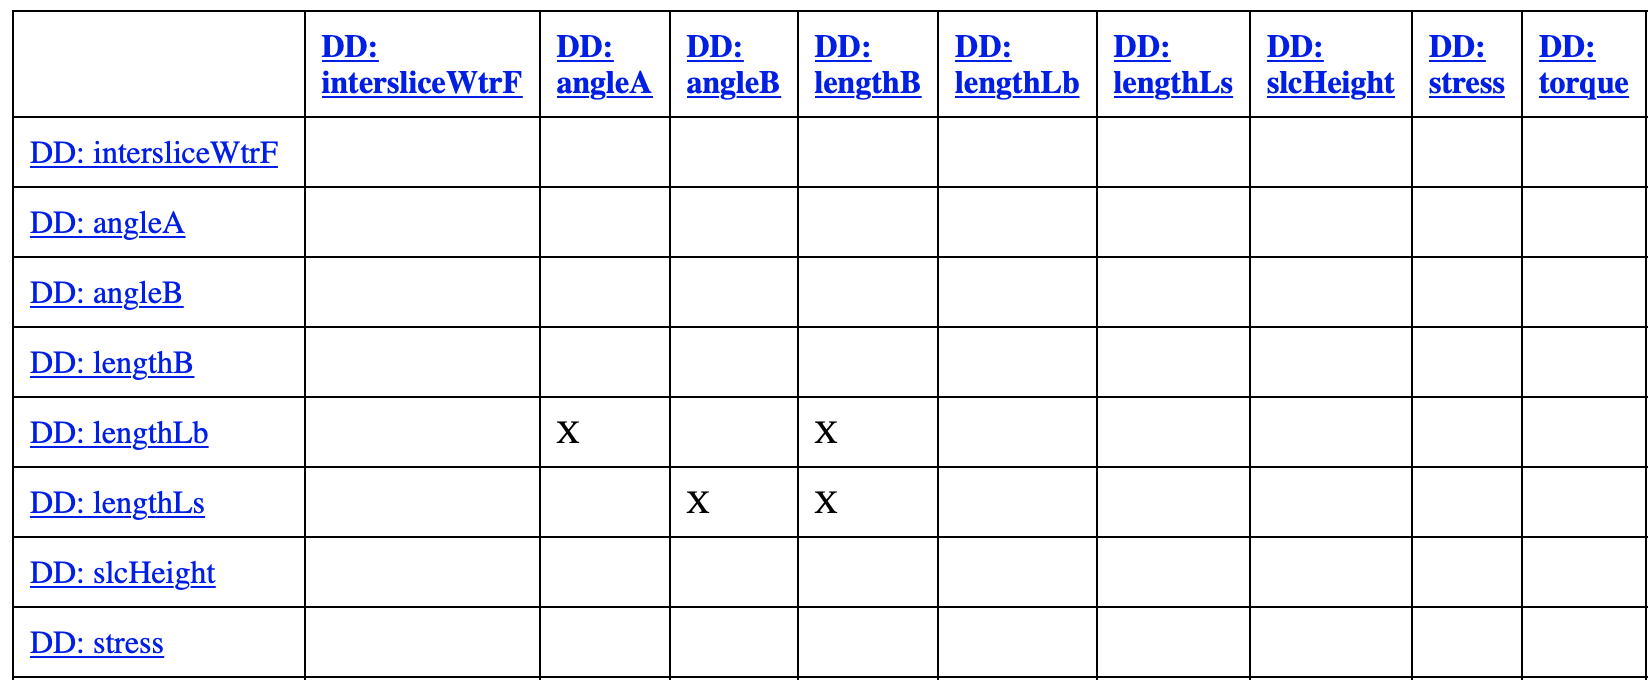
\includegraphics[width=\textwidth]{TraceAfter}
\caption{A portion of an automated traceability matrix constructed with \haskell{traceMatRefinement} in the Drasil example SSP.}\label{fig:traceAfter}
\end{figure}

\noindent matrix --- three traceability matrices maintained\footnote{Not really} manually. The new view functionality for traceability matrices allows the manual matrices to be replaced with automated variants. As the three configurations are common amongst all bundled examples, we encode a function describing each: \haskell[breakanywhere, breakanywheresymbolpre=\textcolor{black}{-}]{traceMatAssumpOther}, \haskell{traceMatRefinement}, and \haskell{traceMatOtherReq}. We encode a convenience function that packages all three together as \haskell{traceMatStandard}. \haskell{traceMatRefinement} replaces at least 50 lines (with the other standard matrices each removing approximately 50 lines each as well) in many bundled examples while producing more accurate output (\autoref{fig:traceAfter}) without requiring manual upkeep. The definition is:

% FIXME: Do items vs items here and as traceAfter since Assumptions aren't supposed to be here at this point....
\begin{tcolorbox}[breakable, toprule at break=0pt, bottomrule at break=0pt]
\begin{minted}{haskell}
traceMatRefinement :: TraceConfig
traceMatRefinement = TraceConfig "TraceMatRefvsRef"
  [plural Doc.dataDefn, plural Doc.thModel, plural
  Doc.genDefn, plural Doc.inModel +:+. S "with each other"]
  (titleize' item +:+ S "and Other" +:+ titleize' section_)
  [tvDataDefns, tvTheoryModels, tvGenDefns, tvInsModels]
  [tvDataDefns, tvTheoryModels, tvGenDefns, tvInsModels]
\end{minted}
\end{tcolorbox}

The implementation of a refined, higher-level \haskell{DocDesc} constructor for traceability matrices improves the display and flexibility of the matrices while moving \haskell{DocDesc} in the correct direction towards a declarative language. 
\clearpage

\section{Removing Boilerplate}\label{dlToDocLang}  % Pulling a fast one here. 

If we implement the desired declarative solution, one where \haskell{DocDesc} is hidden from authors and instead present a cleaner declarative \haskell{SRSDecl}, then we ought to investigate what functions exposed and used within \textit{drasil-example} take \haskell{DocDesc} as an argument. Any function that does will either need to be removed or altered to be used solely within \textit{drasil-docLang} as \haskell{DocDesc} will no longer be available in the sub-package. From \autoref{teExample} we have a set of incantations that take \haskell{DocDesc}, or a sub-structure of \haskell{DocDesc}, as an input:

% Author Note: Handwaving away the table of symbols constructors (ccss) that were lifted to docLang since there is some outstanding work that was out of scope on that.
\begin{tcolorbox}
\begin{minted}{haskell}
label :: TraceMap
label = generateTraceMap thisSRS

refBy :: RefbyMap
refBy = generateRefbyMap label

scs :: SCSSub
scs = getSCSSub thisSRS

dataDefn :: [DataDefinition]
dataDefn = getTraceMapFromDD scs

reqs :: [ReqChunk]
reqs = getTraceMapFromReqs scs

chgs :: [Change]
chgs = getTraceMapFromChgs scs
\end{minted}
\end{tcolorbox}

The desired model where information is contained within \haskell{ChunkDB} and retrieved to populate \haskell{DocDesc} renders \haskell{getSCSSub}, \haskell{getTraceMapFromDD}, \linebreak\haskell{getTraceMapFromReqs}, \haskell{getTraceMapFromChgs}, and others as unneeded. The functions previously served two purposes: gather chunks to populate a \haskell{ChunkDB} and gather chunks that are subsequently consumed for their \haskell{UID}s within \haskell{generateTraceMap}. The functions' use within individual examples is unnecessary and may be removed under the new model of chunk propagation.

The remaining SRS boilerplate within examples is \haskell{generateTraceMap} and \haskell{generateRefbyMap}. Both \haskell{generateTraceMap} and \haskell{generateRefbyMap} are computed from the SRS using \haskell{DocDesc} to populate a table, which are passed as arguments to the \haskell{cdb} constructor.

\haskell{generateTraceMap} is an excellent candidate to relocate to \textit{drasil-docLang}. It is a function that is required for automated traceability matrices to function. It does not provide any means of customization to a user calling it, as it simply extracts chunks from \haskell{DocDesc}. It is truly boilerplate, which users must remember to call. The reason for its existence within each example is because it becomes a table in \haskell{ChunkDB}, which is always constructed for a software system. We would instead like to delay construction of these tables to occur after a \haskell{ChunkDB} has been constructed and during \textit{drasil-docLang} processing of \haskell{DocDesc}. \haskell{generateRefbyMap} transitively depends on the \haskell{DocDesc}, as it inverts the map produced by \haskell{generateTraceMap}, allowing both to be moved together, while \haskell{generateRefbyMap} can be an afterthought to a design for \haskell{generateTraceMap}.

All tables within \haskell{ChunkDB} implement Lenses~\cite{Lenses} allowing for modification after initial construction. If we leverage this existing feature, we can move traceability information generation (and subsequent table updates within \haskell{ChunkDB}) to immediately after \haskell{DocDesc} is constructed. Due to the new information propagation flow this chapter is enacting, traceability information should not be completely available until \haskell{DocDesc} is constructed and refers specifically to the SRS document. If we were to modify which chunks appeared in an SRS (through possible elaboration when constructing \haskell{DocDesc} from \haskell{SRSDecl}) we would like the traceability information to include the most recent data as opposed to ``stale" data from an earlier point in the artefact generation process. Another benefit of delaying traceability information extraction is we remove the need for users to be concerned about how traceability information is gathered and stored and can simplify the \haskell{cdb} constructor to remove the two tables that are later populated.

In an effort to realize the relocation of \haskell{generateTraceMap} and \linebreak\haskell{generateRefbyMap}, we should examine the definition of the candidate destination function, \haskell{mkDoc}, a function that transforms a \haskell{DocDesc} --- when we are done elaborating an \haskell{SRSDecl} --- to a \textit{drasil-lang} \haskell{Document}, ideally behaving as the \textit{drasil-docLang} transformation function. \haskell{mkDoc}'s input is the finalized \haskell{DocDesc} making it an appropriate location to derive traceability information and amend the \haskell{ChunkDB} prior to construction of the traceability matrices. We construct a function, \haskell{fillTraceMaps}, which \haskell{set}s the two traceability related tables after invoking \haskell{generateTraceMap} and \haskell{generateRefbyMap}, and call the function early within \haskell{mkDoc} before any \haskell{DocDesc} constructors are translated to \haskell{Document} constructors.

%\begin{tcolorbox}
%\begin{minted}{haskell}
%mkDoc :: DocDesc -> (IdeaDict -> IdeaDict -> Sentence) ->
%  SystemInformation -> Document
%mkDoc l comb si@SI {_sys = sys, _kind = kind,
%  _authors = authors} = Document
%	(nw kind `comb` nw sys) (foldlList Comma List $
%	  map (S . name) authors) (mkSections si l)
%\end{minted}
%\end{tcolorbox}

%where \haskell{mkSections} translates each \haskell{DocDesc} constructor into a \textit{drasil-lang} \haskell{Section}. At the point where \haskell{mkSections} is called, we have the final \haskell{DocDesc}. If we are to update the \haskell{_sysinfodb} within \haskell{SystemInformation} to contain traceability information, it would include the final state of \haskell{DocDesc}. To perform the action of populating the traceability information named \haskell{fillTraceMaps}, updating \haskell{SystemInformation} according to a \haskell{DocDesc}:

%\begin{tcolorbox}
%\begin{minted}{haskell}
%fillTraceMaps :: DocDesc ->
%  SystemInformation -> SystemInformation
%fillTraceMaps dd si@SI{_sysinfodb = db} = si {_sysinfodb =
%  set refbyTable (generateRefbyMap tdb) $
%  set traceTable tdb db} where
%    tdb = generateTraceMap dd
%\end{minted}
%\end{tcolorbox}
%
%where \haskell{set} is a Lens function to modify the table within the \haskell{ChunkDB} \haskell{db}. Updating \haskell{mkDoc} to populate the traceability tables yields:
%
%\begin{tcolorbox}
%\begin{minted}{haskell}
%mkDoc :: DocDesc -> (IdeaDict -> IdeaDict -> Sentence) ->
%  SystemInformation -> Document
%mkDoc l comb si@SI {_sys = sys, _kind = kind,
%  _authors = authors} = Document
%	(nw kind `comb` nw sys) (foldlList Comma List $
%	  map (S . name) authors)
%	(mkSections (fillTraceMaps l si) l)
%\end{minted}
%\end{tcolorbox}

The last function, although not taking \haskell{DocDesc} as input, is an incantation from \autoref{teExample} requiring migration or removal. The function, \haskell{collectUnits}, requires a list of symbols to determine which units are involved in an SRS and a \haskell{ChunkDB}. It is not mandatory to migrate to \textit{drasil-docLang}; however, the action performed is specifically for a \haskell{DocDesc} section. With the introduction of \haskell{SRSDecl}, this should not be something an author is manually required to perform. \haskell{collectUnits} extracts units from the provided symbols, which are used to display a table of units within the SRS. Similar to the traceability matrix, \haskell{collectUnits}' action is specifically for a section. Failure for a user to perform an action should not result in an inaccurate or empty table of units section, as such, \haskell{collectUnits} should be invoked by \textit{drasil-docLang} as needed to ensure consistency throughout the document and effectively be ``magic" for the system implementor. 

To migrate \haskell{collectUnits} to \textit{drasil-docLang}, we require means to extract the used symbols as opposed to having them explicitly passed by the user. Symbols within \haskell{DocDesc} are contained within \haskell{Sentence}s and \haskell{Expr}essions. Conveniently, two functions exist to scan \haskell{DocDesc} and extract such elements: \haskell{getDocDesc} and \haskell{egetDocDesc}, respectively. Another function (\haskell{ccss'}) exists that extract symbols, contained in \haskell{QuantityDict}, from \haskell{Sentence} and \haskell{Expr}. Combining these components together we have, \haskell[breakanywhere, breakanywheresymbolpre=\textcolor{black}{-}]{extractUnits}, a function that extracts units given a \haskell{DocDesc}:

\begin{tcolorbox}
\begin{minted}{haskell}
extractUnits :: DocDesc -> ChunkDB -> [UnitDefn]
extractUnits dd cdb = collectUnits cdb $
  ccss' (getDocDesc dd) (egetDocDesc dd) cdb
\end{minted}
\end{tcolorbox}

\haskell{extractUnits} allows for the \haskell{collectUnits} boilerplate to be removed from each example. The function is invoked during the expansion of \haskell{DocDesc}'s constructor to produce a table of units. Deferral of unit collection allows it to occur in the function that generates the table of units reducing the surface of functions that know \textit{how} the table of units is generated and concentrate the knowledge in the area of interest.

%\haskell{extractUnits} provides an advantage over the previous user-specified method: it only includes units from symbols which appear in the final SRS. The previous method allowed for an over-specification of symbols leading to entries in the table of units of units which did not appear within the final document. The last step to remove the user-required boilerplate is to use \haskell{extractUnits} when a \haskell{DocDesc} \haskell{TUnit} or \haskell{TUnit'} constructor is specified:

%\begin{tcolorbox}
%\begin{minted}{haskell}
%mkSubRef :: SystemInformation -> RefTab -> Section
%mkSubRef si' TUnits = mkSubRef si' $ TUnits' defaultTUI
%mkSubRef SI {_sysinfodb = db} (TUnits' con) =
%  tableOfUnits (nub $ sortBy compUnitDefn $
%  	extractUnits dd db) (tuIntro con)
%\end{minted}
%\end{tcolorbox}
%
%where \haskell{mkSubRef} populates reference tables when constructing the reference section of the Smith et al. SRS template\cite{smith2005new}, \haskell{compUnitDefn} provides lexicographic-like ordering to units, and \haskell{dd} is a \haskell{DocDesc} from an outer-scope function omitted in the code snippet displayed.

The migration of \haskell{collectUnits} has removed all incantations required for proper SRS function shown in \autoref{teExample} through relocation of many functions to \textit{drasil-docLang}, moving the goal of \haskell{SRSDecl} closer to reality.


\section{More Boilerplate?}\label{dlMultiplate}

In \autoref{diFraming} we made \haskell{DocDesc}'s \haskell{Assumptions} constructor consistent with the other chunk constructors, as \haskell{DocDesc} will soon be hidden within \textit{drasil-docLang}. We ought to address the introspection passes we used in \autoref{dlToDocLang} --- namely \haskell{generateTraceMap}, \haskell{getDocDesc}, and \haskell{egetDocDesc} --- to ensure their inclusion of content present in \haskell{Assumptions}, something that has not been done due to the anomalous constructor.

Repeatedly in this chapter we have discussed the traceability matrix and the enhancements provided, however, the \haskell{Assumptions} constructor has complicated efforts to include \haskell{ConceptInstance}s related to assumptions within the traceability matrix. \haskell{generateTraceMap} extracts traceability information from the SRS, we will use it as a starting point to investigate including assumptions in the matrices. Examining the function shows:

\begin{tcolorbox}
\begin{minted}{haskell}
generateTraceMap :: DocDesc -> TraceMap
generateTraceMap a = Map.unionsWith (\(w,x) (y,z) -> (w ++ y,
  ordering x z)) [traceMap' extractSFromNotes tt,
  traceMap' extractSFromNotes gd,
  traceMap' extractSFromNotes ddef,
  traceMap' extractSFromNotes imod,
  traceMap' extractSFromDeriv gd,
  traceMap' extractSFromDeriv ddef,
  traceMap' extractSFromDeriv imod,
  ...]
  where
    tt   = getTraceMapFromTM $ getSCSSub a
    gd   = getTraceMapFromGD $ getSCSSub a
    imod = getTraceMapFromIM $ getSCSSub a
    ddef = getTraceMapFromDD $ getSCSSub a
    ...
    ordering x y = if x == y then x else error "..."
\end{minted}
\end{tcolorbox}

%where \haskell{extractSFrom} functions extract \haskell{Sentence}s from chunks (following typeclass constraints) and \haskell{traceMap'} extracts references from \haskell{Sentence}s. 

Examining \haskell{getTraceMapFrom} functions reveals:

\begin{tcolorbox}[breakable, toprule at break=0pt, bottomrule at break=0pt]
\begin{minted}{haskell}
getTraceMapFromTM :: [SCSSub] -> [TheoryModel]
getTraceMapFromTM (TMs _ _ t:_) = t
getTraceMapFromTM (_:tl)        = getTraceMapFromTM tl
getTraceMapFromTM []            = error "No TM found."

getTraceMapFromGD :: [SCSSub] -> [GenDefn]
getTraceMapFromGD (GDs _ _ gd _:_) = gd
getTraceMapFromGD (_:tl)           = getTraceMapFromGD tl
getTraceMapFromGD []               = []
\end{minted}
\end{tcolorbox}

Although only two of the functions have been reproduced, all the \haskell[breakanywhere, breakanywheresymbolpre=\textcolor{black}{-}]{getTraceMapFrom} functions follow a similar template. Between the two functions shown, their empty behaviour differs for unexplained reasons. Each function's ``useful" results come from the first pattern match, the other two pattern matches can be seen as structural noise. 

Before continuing with the original idea to include \haskell{Assumptions} in introspective \haskell{DocDesc} passes, we should survey the other two passes to discern whether boilerplate is just as pervasive.

Beginning with \haskell{getDocDesc} we have:

\begin{tcolorbox}
\begin{minted}{haskell}
getDocDesc :: DocDesc -> [Sentence]
getDocDesc = concatMap getDocSec

getDocSec :: DocSection -> [Sentence]
getDocSec (RefSec r)           = getRefSec r
getDocSec (IntroSec i)         = getIntrosec i
getDocSec (StkhldrSec s)       = getStk s
getDocSec (GSDSec g)           = getGSD g
getDocSec (SSDSec s)           = getSSD s
...

getSSD :: SSDSec -> [Sentence]
getSSD (SSDProg ssd) = concatMap getSSDSub ssd

getSSDSub :: SSDSub -> [Sentence]
getSSDSub (SSDProblem pd)    = getProblem pd
getSSDSub (SSDSolChSpec sss) = getSol sss

getProblem :: ProblemDescription -> [Sentence]
getProblem (PDProg s x _) = s : concatMap getSec x

getSol :: SolChSpec -> [Sentence]
getSol (SCSProg x) = concatMap getSCSSub x
...
\end{minted}
\end{tcolorbox}

Observation of the functions shown indicates \haskell{getDocDesc} is simply a fold over \haskell{DocDesc}. Some functions such as \haskell{getSSD} are a simple \haskell{concatMap}! In all the code displayed, comprising a part of \haskell{getDocDesc}, only one line actually extracts a \haskell{Sentence}! The (portion of a) line is the second pattern match of \haskell{getProblem}. The rest is dealing exclusively with traversing the structure. Does \haskell{egetDocDesc} improve on the situation?

\begin{tcolorbox}[breakable, toprule at break=0pt, bottomrule at break=0pt]
\begin{minted}{haskell}
egetSSD :: SSDSec -> [Expr]
egetSSD (SSDProg ssd) = concatMap egetSSDSub ssd

egetSSDSub :: SSDSub -> [Expr]
egetSSDSub (SSDProblem p)   = egetProblem p
egetSSDSub (SSDSolChSpec s) = egetSol s

egetProblem :: ProblemDescription -> [Expr]
egetProblem (PDProg _ s _) = concatMap egetSec s

egetSol :: SolChSpec -> [Expr]
egetSol (SCSProg s) = concatMap egetSCSSub s
\end{minted}
\end{tcolorbox}

A sample of functions called through \haskell{egetDocDesc} demonstrates a similar situation albeit worse. Not only do none of the functions returning \haskell{[Expr]} produce anything of value and only traverse the structure, they omit traversing \haskell{Sentence}s and thus \textbf{miss} all \haskell{Expr}s embedded in \haskell{Sentence}s! \haskell{Sentence}s include a constructor (\haskell{E}) used to embed \haskell{Expr}. This can be observed in the code comprising \haskell{getProblem} and \haskell{egetProblem}, the \haskell{Sentence} extracted in the former is ignored in the latter.

With no framework in place for \haskell{DocDesc} to provide convenient means to add an introspective pass, we impair the desired behaviour for \haskell{DocDesc} to be a structure designed to be interrogated. If it remains as tedious and boilerplate-heavy to introduce a pass, it is entirely possible other developers and maintainers in a rush may ``hack together" a partial (in the functional sense) solution that easily breaks. Further, each introduced pass will inhibit \haskell{DocDesc}'s ability to change and evolve. Developer's desire to alter \haskell{DocDesc} will also be stifled due to the sheer amount of boilerplate requiring modification.

A desirable solution is one that abstracts the boilerplate away, yet allows ``random access" into the substructures that make up \haskell{DocDesc}. Another useful feature would be a mechanism to fold \haskell{DocDesc} as current passes all return a list of \textit{something}. A design with both features would allow for a streamlined re-implementation of the three existing passes and reduce the effort and time to write additional passes. 

% Literally a hack to support a type signature not bound to a function
The solution exists within the Haskell ecosystem as the package Multiplate~\cite{multiplate}. Multiplate provides a typeclass, \haskell{Multiplate}, that when implemented on structure provides the two features (random access, folding) desired. The data structure implementing \haskell{Multiplate} is a record where each field becomes a point of random access. Without delving too far into the details of multiplate, the structure includes a type variable \haskell{f} where each field is a function from \haskell{a ->} \haskell{f} \haskell{a}, relying on applicative functors to aid in the removal of the boilerplate.

Delving straight into Drasil's use of multiplate, we create a data structure \haskell{DLPlate} including a field for each sub-structure of \haskell{DocDesc} exposing the widest surface for random access.

\begin{tcolorbox}[breakable, toprule at break=0pt, bottomrule at break=0pt]
\begin{minted}{haskell}
data DLPlate f = DLPlate {
    docSec :: DocSection -> f DocSection,
    ...
    ssdSec :: SSDSec -> f SSDSec,
    ssdSub :: SSDSub -> f SSDSub,
    pdSec :: ProblemDescription -> f ProblemDescription,
    pdSub :: PDSub -> f PDSub,
    scsSub :: SCSSub -> f SCSSub,
    ...
  }
\end{minted}
\end{tcolorbox}

The \haskell{Multiplate} typeclass requires definitions for two functions \haskell[breakanywhere, breakanywheresymbolpre=\textcolor{black}{-}]{multiplate} and \haskell{mkPlate}. \haskell{multiplate} describes how each data structure relates to each field within the plate. We realize this for \haskell{DLPlate} as:

\begin{tcolorbox}[breakable, toprule at break=0pt, bottomrule at break=0pt]
\begin{minted}{haskell}
instance Multiplate DLPlate where
  multiplate p = DLPlate ds res intro intro' stk stk' gs gs'
    ss ss' pd pd' sc rs rs' lcp ucp ts es acs aps where
    ...
    ds (SSDSec x) = SSDSec <$> ssdSec p x
    ...

    res (RefProg c x) = RefProg <$> pure c <*> pure x
    ...
    ss (SSDProg prog) = SSDProg <$> traverse (ssdSub p) prog
    ss' (SSDProblem prog) = SSDProblem <$> pdSec p prog
    ss' (SSDSolChSpec (SCSProg spec)) = SSDSolChSpec .
      SCSProg <$> traverse (scsSub p) spec
    pd (PDProg s sect progs) = PDProg <$> pure s <*>
      pure sect <*> traverse (pdSub p) progs
    pd' (TermsAndDefs s cs) = TermsAndDefs <$> pure s <*>
      pure cs
    pd' (Goals s ci) = Goals <$> pure s <*> pure ci
    pd' (PhySysDesc nm s lc c) = PhySysDesc <$> pure nm <*>
      pure s <*> pure lc <*> pure c
    sc (Assumptions c) = Assumptions <$> pure c
    sc (TMs s f t) = TMs <$> pure s <*> pure f <*> pure t
    sc (GDs s f g d) = GDs <$> pure s <*> pure f <*>
      pure g <*> pure d
    sc (DDs s f dd d) = DDs <$> pure s <*> pure f <*>
      pure dd <*> pure d
    sc (IMs s f i d) = IMs <$> pure s <*> pure f <*>
      pure i <*> pure d
    sc (Constraints s c) = Constraints <$> pure s <*> pure c
    sc (CorrSolnPpties c cs) = CorrSolnPpties <$> pure c <*>
      pure cs
    ...
\end{minted}
\end{tcolorbox}

Many of the functions alluded to in the first line have been elided for brevity.

The second function required for \haskell{Multiplate} is \haskell{mkPlate}, which takes a function used to construct each field of the completely instantiated plate. For \haskell{DLPlate} this function is implemented as:

\begin{tcolorbox}
\begin{minted}{haskell}
instance Multiplate DLPlate where
  mkPlate b = DLPlate (b docSec) (b refSec) (b introSec)
    (b introSub) (b stkSec) (b stkSub) (b gsdSec) (b gsdSub)
    (b ssdSec) (b ssdSub) (b pdSec) (b pdSub) (b scsSub)
    (b reqSec) (b reqSub) (b lcsSec) (b ucsSec) (b traceSec)
    (b offShelfSec) (b auxConsSec) (b appendSec)
\end{minted}
\end{tcolorbox}

We have completed all the boilerplate required to produce introspection passes for \haskell{DocDesc}!

We begin the task of migrating the existing passes to \haskell{DLPlate}. In the instantiated plates, we make heavy use of the Glasgow Haskell Compiler Haskell language extension \texttt{LambdaCase}\footnote{\url{https://downloads.haskell.org/~ghc/latest/docs/html/users_guide/glasgow_exts.html\#lambda-case}}. \texttt{LambdaCase} introduces syntax sugar allowing replacement of

\begin{tcolorbox}
\begin{minted}{haskell}
\a -> case a of
  p1 -> ...
  p2 -> ...

-- With
\case 
  p1 -> ...
  p2 -> ...
\end{minted}
\end{tcolorbox}

Multiplate provides the function \haskell{foldFor} to fold a plate instantiation into a \haskell{Monoid}. Due to the folding operation performed on the plate, the functor used to realize the type transformation is \haskell{Constant}, defined as\footnote{\url{http://hackage.haskell.org/package/transformers-0.5.6.2/docs/src/Data.Functor.Constant.html\#Constant}}:

\begin{tcolorbox}
\begin{minted}{haskell}
newtype Constant a b = Constant {getConstant :: a}
\end{minted}
\end{tcolorbox}

We begin by implementing a \haskell{DLPlate} to extract ``things" from \haskell{Section}s and \haskell{Content}s within \textit{drasil-lang}'s \haskell{Document} --- as \haskell{DocDesc} contains many constructors including \haskell{Content}s --- which may contain \haskell{Sentence} or \haskell{Expr}. We describe the function with as generic a type as possible, being able to fold \clearpage to any monoid and allowing the caller to specify functions to describe \textit{what} is taken from the two \haskell{Document} types when encountered:

\begin{tcolorbox}
\begin{minted}{haskell}
secConPlate :: Monoid b => (forall a. HasContents a =>
  [a] -> b) -> ([Section] -> b) -> DLPlate (Constant b)
\end{minted}
\end{tcolorbox}

\haskell{(forall a. HasContents a => [a] -> b)} is a second rank type, as the passed function should handle any structure implementing the \haskell{HasContents} typeclass. Glassgow Haskell Compiler requires specifying the \texttt{Rank2Types}\footnote{\url{https://downloads.haskell.org/~ghc/latest/docs/html/users_guide/glasgow_exts.html\#extension-Rank2Types}} language extension for the specified type signature to typecheck. 

Next is to produce a plate observing the sub-structures of interest. The multiplate library includes a function \haskell{purePlate} providing a \haskell{pure} default for each field we do not implement. Further, we would like the \haskell{DocDesc} to be exhaustively folded, requiring either multiplate's \haskell{preorderFold} or \haskell[breakanywhere, breakanywheresymbolpre=\textcolor{black}{-}]{postorderFold}. For the plates being written, the order does not matter, and as such \haskell{preorderFold} has been arbitrarily chosen. Having described the functions required to produce a plate instantiation, we realize \haskell{secConPlate} as:

\begin{tcolorbox}[breakable, toprule at break=0pt, bottomrule at break=0pt]
\begin{minted}{haskell}
secConPlate mCon mSec = preorderFold $ purePlate {
  ...
  gsdSec = Constant <$> \case
    (GSDProg s1 c1 c2 s2) -> mconcat [mSec s1, mCon [c1],
      mCon c2, mSec s2]
    (GSDProg2 _) -> mempty,
  ...
  pdSec = Constant <$> \(PDProg _ s _) -> mSec s,
  pdSub = Constant <$> \case
    (TermsAndDefs _ _) -> mempty
    (PhySysDesc _ _ lc c) -> mCon [lc] `mappend` mCon c
    (Goals _ _) -> mempty,
  ...
}
\end{minted}
\end{tcolorbox}

Many fields have been omitted for brevity. 

With a plate to extract \haskell{Content}s and \haskell{Section}s, we may now describe a plate to extract \haskell{Sentence}s. In a similar manner we keep \haskell{sentencePlate} as abstract by defining it over all \haskell{Monoid}s and including a function to translate \haskell{Sentence} to another type for embedding the plate within another plate. We describe the plate as:
\clearpage
\begin{tcolorbox}
\begin{minted}{haskell}
sentencePlate :: Monoid a =>
  ([Sentence] -> a) -> DLPlate (Constant a)
sentencePlate f = appendPlate
  (secConPlate (f . concatMap getCon') $
    f . concatMap getSec) $
  preorderFold $ purePlate {
    ...
    stkSec = Constant . f <$> \case
      (StkhldrProg _ s) -> [s]
      _ -> [],
    stkSub = Constant . f <$> \case
      (Client _ s) -> [s]
      (Cstmr _) -> [],
    pdSec = Constant . f <$> \(PDProg s _ _) -> [s],
    ...
    scsSub = Constant . f <$> \case
      (Assumptions c) -> map (^. defn) c
      ...
\end{minted}
\end{tcolorbox}

We include \haskell{secConPlate} with \haskell{sentencePlate} as \haskell{Document} constructs embed \haskell{Sentence}s. \haskell{getCon'} and \haskell{getSec} are functions to extract \haskell{Sentence}s from the \haskell{Document} constructs. Similar to the previous plate, we have omitted many fields for brevity. Of interest is the \haskell{pdSec} field that provides the same functionality as \haskell{getProblem} from the previous implementation, but without the boilerplate. Further, we have included \haskell{Assumption} in the new plate beginning to address the original purpose for examining the introspective passes. The final step is using the \haskell{sentencePlate} in \haskell{getDocDesc}:

\begin{tcolorbox}
\begin{minted}{haskell}
fmGetDocDesc :: DLPlate (Constant [a]) -> DocDesc -> [a]
fmGetDocDesc p = concatMap (foldFor docSec p)

getDocDesc :: DocDesc -> [Sentence]
getDocDesc = fmGetDocDesc (sentencePlate id)
\end{minted}
\end{tcolorbox}

\haskell{foldFor} folds \haskell{DLPlate} starting with the \haskell{docSec} field (the top-level structure) and strips the \haskell{Constant} functor off the result.

We repeat the same process as \haskell{sentencePlate} for \haskell{Expr}:

\begin{tcolorbox}[breakable, toprule at break=0pt, bottomrule at break=0pt]
\begin{minted}{haskell}
exprPlate :: DLPlate (Constant [Expr])
exprPlate = sentencePlate (concatMap sentToExp) `appendPlate`
  secConPlate (concatMap egetCon')
  (concatMap egetSec) `appendPlate`
  (preorderFold $ purePlate {
    scsSub = Constant <$> \case
      (TMs _ _ t) -> let r = concatMap (
                             \x -> x ^. invariants ++
                                defExp (x ^. defined_quant ++
                                x ^. defined_fun) ++
                             r (x ^. valid_context)) in r t
      (DDs _ _ d _) -> map sy d ++ defExp d
      (GDs _ _ g _) -> expRel g
      (IMs _ _ i _) -> expRel i
      _ -> [],
    auxConsSec = Constant <$>
      \(AuxConsProg _ qdef) -> defExp qdef
  })where
    defExp :: DefiningExpr a => [a] -> [Expr]
    defExp = map (^. defnExpr)
    expRel :: ExprRelat a => [a] -> [Expr]
    expRel = map (^. relat)
\end{minted}
\end{tcolorbox}

\haskell{sentToExp} extracts any \haskell{Expr}s from \haskell{Sentence}s. \haskell{exprPlate} is only 10 lines longer (and displayed in full) than the snippet showing the previous \haskell{Expr} introspection pass, which contained only boilerplate. \haskell{exprPlate} also remedies the the previous method missing extraction of expressions from \haskell{Sentence}s. Any \haskell{Sentence} extracted by \haskell{sentencePlate} has any \haskell{Expr}s extracted without knowing where the sentences are! 

Similar to \haskell{getDocDesc}, \haskell{egetDocDesc} becomes:

\begin{tcolorbox}
\begin{minted}{haskell}
egetDocDesc :: DocDesc -> [Expr]
egetDocDesc = fmGetDocDesc exprPlate
\end{minted}
\end{tcolorbox}

Finally, we are back to where we started, adding \haskell{Assumptions} to the traceability information. We combine this addition with an introspection pass extracting what each chunk traces to:

\begin{tcolorbox}[breakable, toprule at break=0pt, bottomrule at break=0pt]
\begin{minted}{haskell}
dependencyPlate :: DLPlate (Constant [(UID, [UID])])
dependencyPlate = preorderFold $ purePlate {
  ...
  scsSub = Constant <$> \case
    (Assumptions a) -> getDependenciesOf [defs] a
    ...
    (DDs _ _ d _) -> getDependenciesOf ... d
    (GDs _ _ g _) -> getDependenciesOf ... g
    (IMs _ _ i _) -> getDependenciesOf ... i
    _ -> [],
  ...
} where
  getDependenciesOf :: HasUID a => [a -> [Sentence]] ->
    [a] -> [(UID, [UID])]
  getDependenciesOf fs = map (\x -> (x ^. uid,
    concatMap (lnames' . ($ x)) fs))
  defs :: Definition a => a -> [Sentence]
  defs x = [x ^. defn]
  ...

generateTraceMap :: [DocSection] -> TraceMap
generateTraceMap = traceMap .
  concatMap (foldFor docSec dependencyPlate)
\end{minted}
\end{tcolorbox}

\haskell{lnames'} extracts references from \haskell{Sentence}s. While some chunks have been elided for brevity, it is clear this is much cleaner than the previous implementation. Further, adding dependencies of \haskell{Assumptions} required only a single line of code heavily reducing the effort to add additional constructors and chunks to the traceability matrix.

What began as a simple task to add \haskell{Assumptions} to traceability matrices quickly revealed the complexity and tedium required to interrogate \haskell{DocDesc}. The effort required did not align with the desired model of document processing we have in mind for \textit{drasil-docLang}. To remedy the issue, we leveraged multiplate to abstract away the boilerplate and provide clean, random-access introspection to \haskell{DocDesc}.

\section{\haskell{SRSDecl}}\label{dlSRSDecl}
With \haskell{dependencyPlate} implemented, we have achieved what we set out to perform and completed all the refactoring work necessary for \haskell{DocDesc} to be information complete while giving way to \haskell{SRSDecl} to be the declarative exposed language of SRS documents.

Due to \haskell{SRSDecl} and \haskell{DocDesc} being closely related at the moment, we leverage \haskell{DocDesc} when implementing \haskell{SRSDecl} to ease the expansion process. This allows both data structures to share many sub-structures (which do not differ) making the transformation only that of using the appropriate constructor. 

We provide the outer most data structure of \haskell{SRSDecl} to demonstrate the level of overlap with the \haskell{DL} prefix indicating the data structure is that of \haskell{DocDesc}:

\begin{tcolorbox}
\begin{minted}{haskell}
type SRSDecl = [DocSection]

data DocSection = RefSec DL.RefSec
                | IntroSec DL.IntroSec
                | StkhldrSec DL.StkhldrSec
                | GSDSec DL.GSDSec
                | SSDSec SSDSec
                | ReqrmntSec ReqrmntSec
                | LCsSec
                | UCsSec
                | TraceabilitySec DL.TraceabilitySec
                | AuxConstntSec DL.AuxConstntSec
                | Bibliography
                | AppndxSec DL.AppndxSec
                | OffShelfSolnsSec DL.OffShelfSolnsSec
\end{minted}
\end{tcolorbox}

For brevity we examine the \haskell{SRSDecl} \haskell{SCSSub} (a substructure of \haskell{SSDSec}) that exhibits all behavioural features of \haskell{SRSDecl}'s transformation we wish to show:

% Author Note: Un-GADTed
\begin{tcolorbox}
\begin{minted}{haskell}
data SCSSub = Assumptions
  | TMs [Sentence] Fields
  | GDs [Sentence] Fields DL.DerivationDisplay
  | DDs [Sentence] Fields DL.DerivationDisplay
  | IMs [Sentence] Fields DL.DerivationDisplay
  | Constraints Sentence [UncertainChunk]
  | CorrSolnPpties [ConstrainedChunk] [Contents]
\end{minted}
\end{tcolorbox}

The \haskell{Constraints} and \haskell{CorrSolnPpties} constructors continue to contain an explicit list of chunks as the chunks specified are not stored with full information within \haskell{ChunkDB}. The only required expansion operation, for the other constructors in \haskell{SCSSub}, is to look up chunks in a table of \haskell{ChunkDB} and provide the ordered list of chunks as an argument to the \haskell{DocDesc} constructor. The chunks implemented as \haskell{ConceptInstance} contain a second step similar to \autoref{dlTraceMat} requiring domain filtering to obtain the correct list of chunks. The chunks passed to the \haskell{DocDesc} constructors are in the order they were inserted into \haskell{ChunkDB}, allowing the author to control the display order of the chunks and matching the ordering in all locations where they appear, such as the traceability matrices.

The final step is to adapt \haskell{mkDoc} for \haskell{SRSDecl}. \haskell{mkDoc} takes as input \haskell{SRSDecl}, elaborating the structure to \haskell{DocDesc} before proceeding with document processing as before. The previous infrastructure work performed in this chapter have made the inclusion of \haskell{SRSDecl} rather trivial.

%The first five constructors all expand gathering chunks from \haskell{ChunkDB} to populate the equivalent constructor with \haskell{DocDesc}. We realize this transformation through:

%\begin{tcolorbox}
%\begin{minted}{haskell}
%mkDocDesc :: ChunkDB -> SRSDecl -> DocDesc
%mkDocDesc cdb = map sec where
%  sec :: DocSection -> DL.DocSection
%  sec (RefSec r) = DL.RefSec r
%  sec (IntroSec i) = DL.IntroSec i
%  sec (StkhldrSec s) = DL.StkhldrSec s
%  sec (GSDSec g) = DL.GSDSec g
%  sec (SSDSec (SSDProg s)) = DL.SSDSec $ DL.SSDProg $
%    map ssdSec s
%  ...
%  scsSub :: SCSSub -> DL.SCSSub
%  scsSub Assumptions = DL.Assumptions $
%    fromConcInsDB assumpDom
%  scsSub (TMs s f) = DL.TMs s f $
%    allInDB theoryModelTable
%  ...
%  scsSub (Constraints s c) = DL.Constraints s c
%  scsSub (CorrSolnPpties c cs) = DL.CorrSolnPpties c cs
%  ...
%  expandFromDB :: ([a] -> [a]) ->
%    Getting (UMap a) ChunkDB (UMap a) -> [a]
%  expandFromDB f = f . asOrderedList . (cdb ^.)
%  allInDB :: Getting (UMap a) ChunkDB (UMap a) -> [a]
%  allInDB = expandFromDB id
%  fromConcInsDB :: Concept c => c -> [ConceptInstance]
%  fromConcInsDB c = expandFromDB
%    (filter (\x -> sDom (cdom x) == c ^. uid))
%    conceptinsTable
%\end{minted}
%\end{tcolorbox}
%
%While many lines comprise the transformation, there is no need for a plate on \haskell{SRSDecl} as this is the only transformation to occur with no introspection being involved. Further because many lines are functionally similar to those displayed, they have been omitted. The first four pattern matches to \haskell{sec} show the one-to-one mapping between \haskell{SRSDecl} sub-structures and \haskell{DocDesc}. The \haskell{Assumptions} pattern match functions exactly as described in \autoref{ciFinale}. To achieve the two types of chunk extraction from \haskell{ChunkDB}, we describe a function \haskell{expandFromDB} to extract an entire table from the database. Due to \haskell{ConceptInstance} using domains to differentiate we provide two convenience functions for the \haskell{mkDocDesc} pass, with \haskell{fromConcInsDB} filtering the the table results to only include those of a particular domain. 

%The final step is to use \haskell{mkDocDesc} from \haskell{mkDoc} to make \haskell{DocDesc} transparent to the end-user. We update \haskell{mkDoc} to:

%\begin{tcolorbox}
%\begin{minted}{haskell}
%mkDoc :: SRSDecl -> (IdeaDict -> IdeaDict -> Sentence) ->
%  SystemInformation -> Document
%mkDoc dd comb si@SI {_sys = sys, _kind = kind,
%  _authors = authors, _sysinfodb = db} =
%  Document (nw kind `comb` nw sys)
%  (foldlList Comma List $ map (S . name) authors) $
%  mkSections (fillTraceMaps l si) l where
%    l = mkDocDesc db dd  -- Changed
%\end{minted}
%\end{tcolorbox}

\section{A Plateful of Changes}\label{dlDone}
Many tangents were explored to realize a declarative SRS document language. We enhanced and refined the traceability matrix creation and display. The enhanced version requires less incantations to construct a traceability section and provides flexibility to describe what, and in what order, to produce a traceability matrix. We modified the constructor to be less layout-oriented and specifying the same opaque chunk of layout in multiple places and replaced it with means to describe the matrices themselves using high-level knowledge.

We further removed boilerplate incantations an author must specify to generate a correct SRS. In some cases such as \haskell{getTraceMapFrom} we were able to remove them entirely, while in cases such as \haskell{generateTraceMap} we moved the invocation to \textit{drasil-docLang}. From the boilerplate removed we save 23 lines in \autoref{teExample}, and at least 6 in every bundled example with as many as 26 lines being removed. 

% 29+146+42+12
% 12+49+14+100+14+123+44
Through examination of existing passes we observed a lot of repetitive boilerplate to realize the passes. By leveraging the multiplate~\cite{multiplate} package we were able to obtain passes that produced more accurate data and were simpler to implement. Re-implementing all passes with multiplate and \haskell{DLPlate} added 229 lines of code total with 146 being the definition of \haskell{Multiplate} (meaning only 83 for all the passes combined) while removing the previous passes reduced code by 356 lines.

While the language of \haskell{SRSDecl} is similar to \haskell{DocDesc}, by exposing only \haskell{SRSDecl} we have removed opportunities for users to provide inconsistent information and receive an inconsistent artefact. The languages are likely to diverge to a greater extent as \textit{drasil-docLang} evolves to further enforce consistency and usability. The change itself took longer than expected with many detours fixing deficiencies previously ``accepted" by Drasil developers and users. 

The combination of intermediary data structures and introspection is something we hope becomes more common in other Drasil sub-packages. If introspection is a desired feature within other sub-packages, we hope implementors will look to \textit{drasil-docLang} as the standard for introspection design, following its steps by leveraging multiplate.

% Issues:
% Thoughts on Thunks: https://github.com/JacquesCarette/Drasil/issues/1631
% Whacking Many Moles: https://github.com/JacquesCarette/Drasil/issues/1164
% DocLang Construction Consistency: https://github.com/JacquesCarette/Drasil/issues/1023

% Conclusion:
% Removed n lines of example boilerplate
% Removed n lines of pass boilerplate
% Simplified SRS description while removing footguns
% Expanded traceability matrix versatility while ensuring consistency and making the output more logically organized.